\begin{frame}
	\frametitle{Fala imaginada}
	\only<1>{
		\par A fala imaginada é um fenômeno em que uma pessoa "ouve" a si mesma falando internamente, sem produzir som. As regiões cerebrais usadas na fala imaginada são similares às que estão envolvidas na fala verbal, englobando áreas do córtex motor e pré-motor, além de outras áreas associadas à linguagem e a fala.
		
		\par A ativação cerebral durante processos linguísticos (incluindo a fala imaginada) envolve as seguintes regiões \cite{pinto2012manual}, \cite{Vanderah2020}, \cite{kenhub}:
		
		\begin{itemize}
			\item \textbf{área de Broca}: Produção da fala.
			\item \textbf{área de Wernicke}: Compreensão da linguagem.
			\item \textbf{córtex motor e pré-motor}: Articulação da fala.
			\item \textbf{giro supramarginal}: Planejamento motor da fala.
			\item \textbf{giro supratemporal e médio}: Compreensão linguística e articulação durante a repetição de sílabas.
		\end{itemize}
	}
	\only<2>{
		\framesubtitle{Visão geral do telencéfalo}
		\begin{figure}[p]
			\centering
			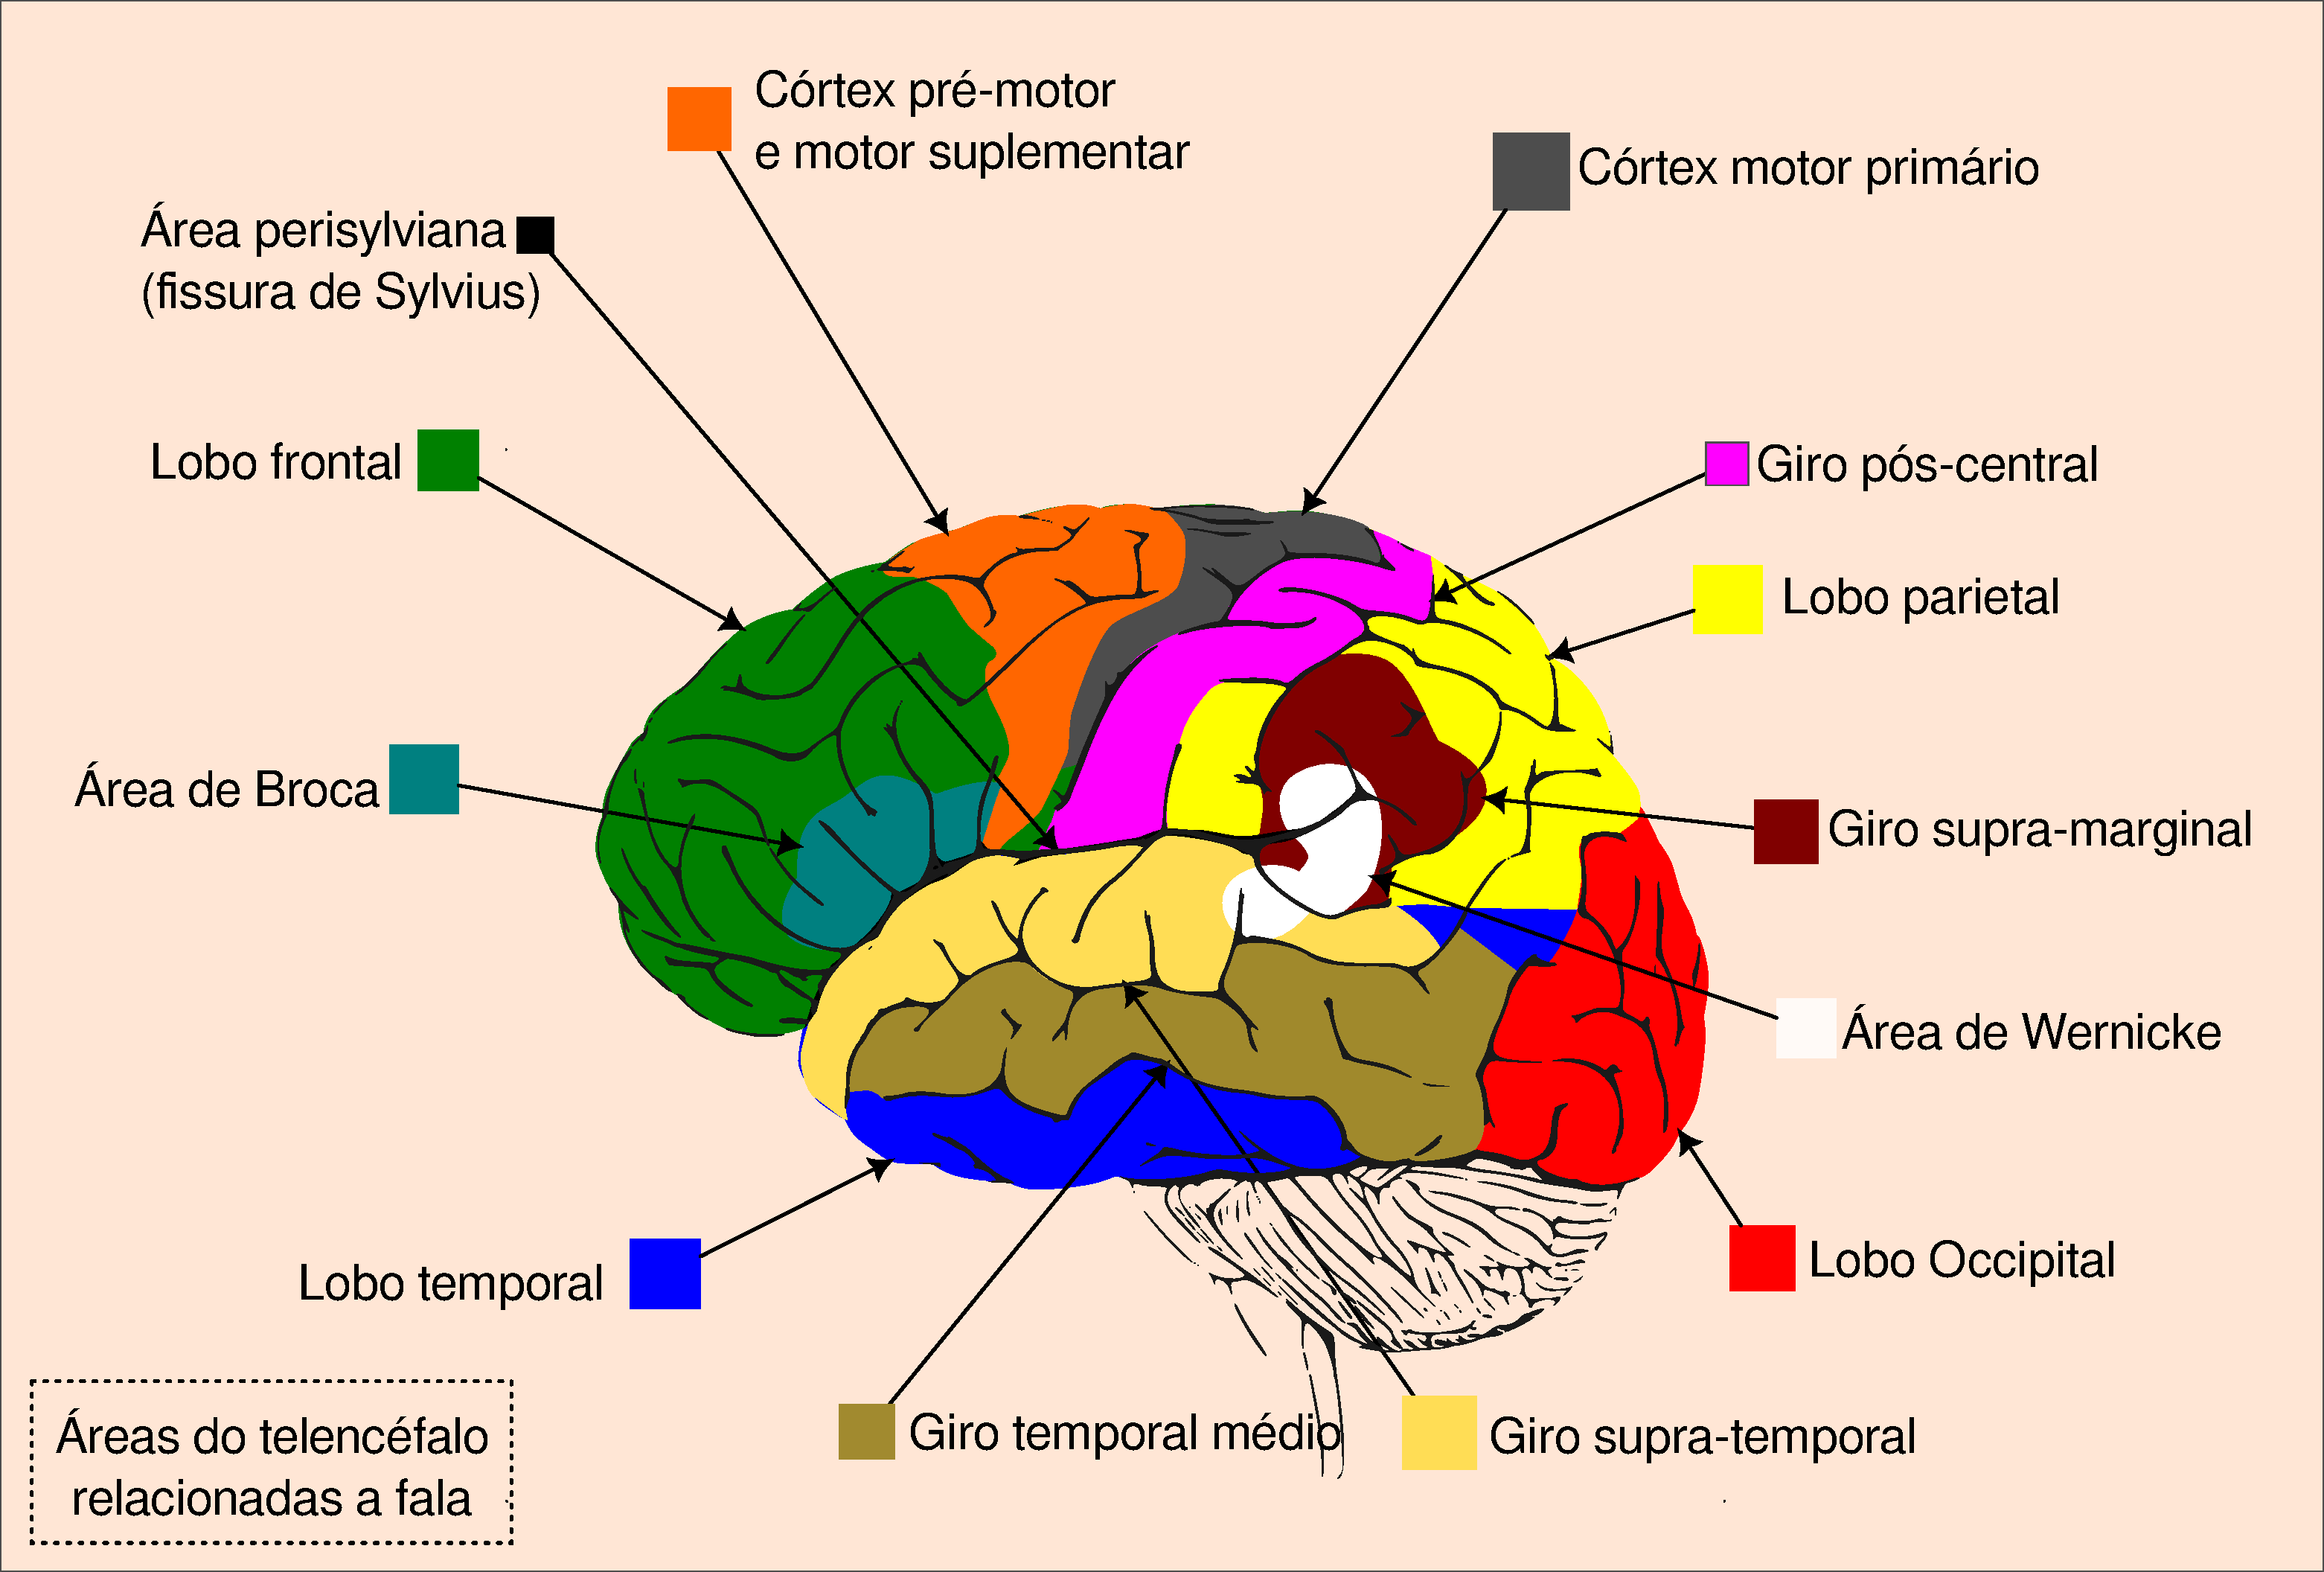
\includegraphics[width=.65\paperwidth,keepaspectratio]{../monography/images/teleencefaloTudo}
			\label{fig:teleencefalotudo}
		\end{figure}
	}
\end{frame}